\chapter{Linear inequalities}
% SECTION HEADER
\rhead{7}
\lhead{Linear inequalities}
%%%% START
\section{Introduction}
An equality states that two values are not equal. In mathematics, we read inequality from left to side, using these symbols:
\begin{align*}
            >&  &   &\textit{Greater than}\\
            <&  &   &\textit{Less than}\\
            \ge&    &   &\textit{Greater than or equal to}\\
            \le&    &   &\textit{Less than or equal to}
\end{align*}
% ============ SECTION
\section{Linear inequality}
In an inequality, we stating both sides of the equation are not equal to each other. It can also be seen as an order relation; that is, it tells us which one of the two expressions is smaller, or larger, than the other one.\\
For example, $x\ge3$ means that $x$ can be 3 or any real numbers greater than $3$. Another example is $0.2x+120\le 120$.\\
Solving an inequality is the process of finding the set of numbers that satisfies the inequality. We have 3 ways to represent the solution set of an inequality
\begin{enumerate}
    \item Set-builder notation
    \item Interval notation
    \item Graphing
\end{enumerate}
We have discussed set-builder notation in chapter 0. We begin this section by looking at interval notation.
% ======== SUBSECTION
\subsection{Interval notation}

Suppose that $a$ and $b$ are real numbers such that $a<b$.
We use two symbols: parentheses $\bm{(\ )}$ and brackets $\bm{[\ \ ]}$:
\begin{itemize}
    \item $\bm{(\ )}$ is used for less than, $<$, or greater than, $>$. This means that specified values for $a$ or $b$ \textbf{are not included}.
    \item $\bm{[\ \ ]}$ is used for less than or equal to, $\le$, or greater than or equal to, $\ge$. This means that specified values for $a$ or $b$ \textbf{are included}.
\end{itemize}

\begin{table}[!ht]
  \caption{Intervals on real numbers}
  \begin{tabularx}{\textwidth}{C{4.2cm}C{3cm}Y}
  \toprule
  %%
  \textbf{Set-builder notation} & \textbf{Interval notation} & \textbf{Graph} \\\midrule
  %%%%
  $\{x \mid a<x<b \}$ & $(a,b)$ &
 {\begin{tikzpicture}[xscale=7, yscale=5, baseline=(current bounding box.west)]
    \draw[->, thick] (0,0) -- (0.5,0);
    \foreach \x/\xtext in {0.1/$a$,0.4/$b$}
    \draw (\x,0.5pt) -- (\x,-0.5pt) node[below] at (\x,-0.05) {\xtext};
    \draw (0.55,0.1pt) node {$x$};
    \draw[(-), ultra thick, blue] (0.1,0) -- (0.4,0);
    \end{tikzpicture}}\\ \midrule
    %%%%
    $\{x \mid a\le x \le b \}$ & $[a,b]$ &
    {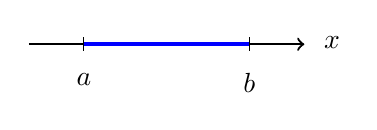
\begin{tikzpicture}[xscale=7, yscale=5, baseline=(current bounding box.west)]
    \draw[->, thick] (0,0) -- (0.5,0);
    \foreach \x/\xtext in {0.1/$a$,0.4/$b$}
    \draw (\x,0.5pt) -- (\x,-0.5pt) node[below] at (\x,-0.05) {\xtext};
    \draw (0.55,0.1pt) node {$x$};
    \draw[{[-]}, ultra thick, blue] (0.1,0) -- (0.4,0);
    \end{tikzpicture}}\\ \midrule
    %%%%%
        $\{x \mid a\le x < b \}$ & $[a,b)$ &
    {\begin{tikzpicture}[xscale=7, yscale=5, baseline=(current bounding box.west)]
    \draw[->, thick] (0,0) -- (0.5,0);
    \foreach \x/\xtext in {0.1/$a$,0.4/$b$}
    \draw (\x,0.5pt) -- (\x,-0.5pt) node[below] at (\x,-0.05) {\xtext};
    \draw (0.55,0.1pt) node {$x$};
    \draw[{[-)}, ultra thick, blue] (0.1,0) -- (0.4,0);
    \end{tikzpicture}}\\ \midrule
    %%%%%
    $\{x \mid a< x \le  b \}$ & $(a,b]$ &
    {\begin{tikzpicture}[xscale=7, yscale=5, baseline=(current bounding box.west)]
    \draw[->, thick] (0,0) -- (0.5,0);
    \foreach \x/\xtext in {0.1/$a$,0.4/$b$}
    \draw (\x,0.5pt) -- (\x,-0.5pt) node[below] at (\x,-0.05) {\xtext};
    \draw (0.55,0.1pt) node {$x$};
    \draw[{(-]}, ultra thick, blue] (0.1,0) -- (0.4,0);
    \end{tikzpicture}}\\ \midrule
    %%%%%
     $\{x \mid x > a \}$ & $(a,+\infty)$ &
    {\begin{tikzpicture}[xscale=7, yscale=5, baseline=(current bounding box.west)]
    \draw[->, thick] (0,0) -- (0.5,0);
    \foreach \x/\xtext in {0.1/$a$}
    \draw (\x,0.5pt) -- (\x,-0.5pt) node[below] at (\x,-0.05) {\xtext};
    \draw (0.55,0.1pt) node {$x$};
    \draw[{(->}, ultra thick, blue] (0.1,0) -- (0.5,0);
    \end{tikzpicture}}\\ \midrule
    %%%%%
     $\{x \mid x \ge a \}$ & $[\, a,+\infty)$ &
    {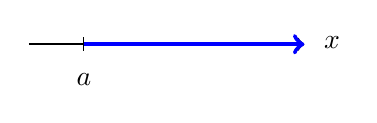
\begin{tikzpicture}[xscale=7, yscale=5, baseline=(current bounding box.west)]
    \draw[->, thick] (0,0) -- (0.5,0);
    \foreach \x/\xtext in {0.1/$a$}
    \draw (\x,0.5pt) -- (\x,-0.5pt) node[below] at (\x,-0.05) {\xtext};
    \draw (0.55,0.1pt) node {$x$};
    \draw[{[->}, ultra thick, blue] (0.1,0) -- (0.5,0);
    \end{tikzpicture}}\\ \midrule
    %%%%%
     $\{x \mid x < b \}$ & $(-\infty,\,b\,)$ &
    {\begin{tikzpicture}[xscale=7, yscale=5, baseline=(current bounding box.west)]
    \draw[->, thick] (0,0) -- (0.5,0);
    \foreach \x/\xtext in {0.4/$b$}
    \draw (\x,0.5pt) -- (\x,-0.5pt) node[below] at (\x,-0.05) {\xtext};
    \draw (0.55,0.1pt) node {$x$};
    \draw[{<-)}, ultra thick, blue] (0,0) -- (0.4,0);
    \end{tikzpicture}}\\ \midrule
    %%%%%
     $\{x \mid x \le b \}$ & $(-\infty,\,b\, ]$ &
    {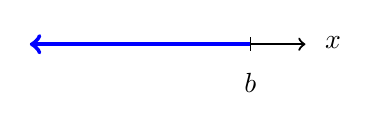
\begin{tikzpicture}[xscale=7, yscale=5, baseline=(current bounding box.west)]
    \draw[->, thick] (0,0) -- (0.5,0);
    \foreach \x/\xtext in {0.4/$b$}
    \draw (\x,0.5pt) -- (\x,-0.5pt) node[below] at (\x,-0.05) {\xtext};
    \draw (0.55,0.1pt) node {$x$};
    \draw[{<-]}, ultra thick, blue] (0,0) -- (0.4,0);
    \end{tikzpicture}}\\ \midrule
    %%%%%
     $\{x \mid x \in \mathbb{R} \}$ & $(-\infty,\,+\infty)$ &
    {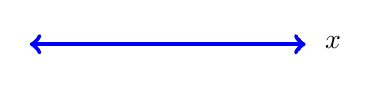
\begin{tikzpicture}[xscale=7, yscale=5, baseline=(current bounding box.west)]
    \draw[->, thick] (0,0) -- (0.5,0);
    \draw (0.55,0.1pt) node {$x$};
    \draw[{<->}, ultra thick, blue] (0,0) -- (0.5,0);
    \end{tikzpicture}}\\ \bottomrule
\end{tabularx}
\end{table}
%
We use $\bm{+\infty}$ to signify that the values continue getting larger without end (unbounded to the right
on the number line). On the other hand, $\bm{-\infty}$ signify that the values continue getting smaller without end (unbounded to the left on the number line).
% ====== EXAMPLE 1
\begin{exa}
    Express each interval in set-builder notation and graph.\\
    a. $[-2,\,5)$\\
    b. $[1,\,3.5]$\\
    c. $(-\infty,\,-1)$
\end{exa}
    It's get easier if we convert them into set-builder notation first.\\
    a. $[-2,\,5) = \{x \mid -2\le x<5\}$
    \begin{center}
    \begin{tikzpicture}[xscale=0.7]
    \draw[->, thick] (-6,0) -- (6,0);
    \foreach \x in  {-5,...,5}
    \draw[shift={(\x,0)},color=black] (0pt,3pt) -- (0pt,-3pt);
    \foreach \x in {-5,...,5}
    \draw[shift={(\x,0)},color=black] (0pt,0pt) -- (0pt,-3pt) node[below] {$\x$};
    \draw (6.4,0.1pt) node {$x$};
    \draw[{[-)}, ultra thick, blue] (-2,0) -- (5,0);
    \end{tikzpicture}
    \end{center}
    % part b
        b. $[1,\,3.5] = \{x \mid 1\le x \le 3.5\}$
    \begin{center}
    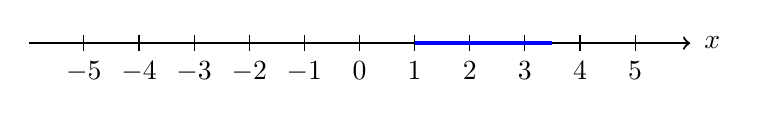
\begin{tikzpicture}[xscale=0.7]
    \draw[->, thick] (-6,0) -- (6,0);
    \foreach \x in  {-5,...,5}
    \draw[shift={(\x,0)},color=black] (0pt,3pt) -- (0pt,-3pt);
    \foreach \x in {-5,...,5}
    \draw[shift={(\x,0)},color=black] (0pt,0pt) -- (0pt,-3pt) node[below] {$\x$};
    \draw (6.4,0.1pt) node {$x$};
    \draw[{[-]}, ultra thick, blue] (1,0) -- (3.5,0);
    \end{tikzpicture}
    \end{center}
    % part c
        c. $(-\infty,\,-1) = \{x \mid x<-1\}$
    \begin{center}
    \begin{tikzpicture}[xscale=0.7]
    \draw[->, thick] (-6,0) -- (6,0);
    \foreach \x in  {-5,...,5}
    \draw[shift={(\x,0)},color=black] (0pt,3pt) -- (0pt,-3pt);
    \foreach \x in {-5,...,5}
    \draw[shift={(\x,0)},color=black] (0pt,0pt) -- (0pt,-3pt) node[below] {$\x$};
    \draw (6.4,0.1pt) node {$x$};
    \draw[{<-)}, ultra thick, blue] (-5.6,0) -- (-1,0);
    \end{tikzpicture}
    \end{center}
% ======== SUBSECTION
\subsection{Intersections and unions}
Consider two intervals $A$ and $B$. The common portion of two intervals $A$ and $B$ is called \textit{intersection} of $A$ and $B$ and it's denoted as $A \cap B$.\\
The merge of two intervals $A$ and $B$, however, is called the \textit{union} of $A$ and $B$ and it's denoted as $A \cup B$.\\
For example, let's take a look at two intervals $(-\infty,\,4)$ and $[3,\,5]$ 
    \begin{center}
    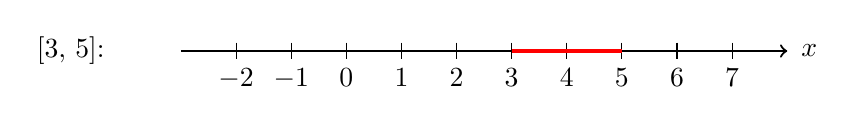
\begin{tikzpicture}[xscale=0.7]
    \draw[->, thick] (-3,0) -- (8,0);
    \foreach \x in  {-2,...,7}
    \draw[shift={(\x,0)},color=black] (0pt,3pt) -- (0pt,-3pt);
    \foreach \x in {-2,...,7}
    \draw[shift={(\x,0)},color=black] (0pt,0pt) -- (0pt,-3pt) node[below] {$\x$};
    \draw (8.4,0.1pt) node {$x$};
    \draw (-5,0.1pt) node {$[3,\,5]$:};
    \draw[{[-]}, ultra thick, red] (3,0) -- (5,0);
    \end{tikzpicture}
    \end{center}
%%%%%
    \begin{center}
    \begin{tikzpicture}[xscale=0.7]
    \draw[->, thick] (-3,0) -- (8,0);
    \foreach \x in  {-2,...,7}
    \draw[shift={(\x,0)},color=black] (0pt,3pt) -- (0pt,-3pt);
    \foreach \x in {-2,...,7}
    \draw[shift={(\x,0)},color=black] (0pt,0pt) -- (0pt,-3pt) node[below] {$\x$};
    \draw (8.4,0.1pt) node {$x$};
    \draw (-5,0.1pt) node {$(-\infty,\,4)$:};
    \draw[{<-)}, ultra thick, blue] (-2.5,0) -- (4,0);
    \end{tikzpicture}
    \end{center}
Intersection and union of these two intervals are
\begin{equation*}
    (-\infty,\,4) \cap [3,\,5]=[3,\,4)
\end{equation*}
    \begin{center}
    \begin{tikzpicture}[xscale=0.7]
    \draw[->, thick] (-3,0) -- (8,0);
    \foreach \x in  {-2,...,7}
    \draw[shift={(\x,0)},color=black] (0pt,3pt) -- (0pt,-3pt);
    \foreach \x in {-2,...,7}
    \draw[shift={(\x,0)},color=black] (0pt,0pt) -- (0pt,-3pt) node[below] {$\x$};
    \draw (8.4,0.1pt) node {$x$};
    \draw[{[-)}, ultra thick, green] (3,0) -- (4,0);
    \end{tikzpicture}
    \end{center}
\begin{equation*}
    (-\infty,\,4) \cup [3,\,5] = (-\infty,\,5]
\end{equation*}
    \begin{center}
    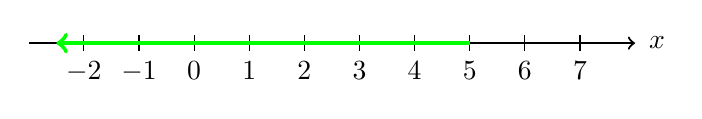
\begin{tikzpicture}[xscale=0.7]
    \draw[->, thick] (-3,0) -- (8,0);
    \foreach \x in  {-2,...,7}
    \draw[shift={(\x,0)},color=black] (0pt,3pt) -- (0pt,-3pt);
    \foreach \x in {-2,...,7}
    \draw[shift={(\x,0)},color=black] (0pt,0pt) -- (0pt,-3pt) node[below] {$\x$};
    \draw (8.4,0.1pt) node {$x$};
    \draw[{<-]}, ultra thick, green] (-2.5,0) -- (5,0);
    \end{tikzpicture}
    \end{center}
% ====== EXAMPLE 2
\begin{exa}
    Use graphs to find each set:\\
    a. $[1,\,3] \cap (2,6)$\hspace{1cm} b. $[1,\, 3] \cup (2,6)$
\end{exa}
a. The intersection of the intervals $[1,\,3]$ and $(2,6)$ consists of the numbers that are in both intervals.
    \begin{center}
    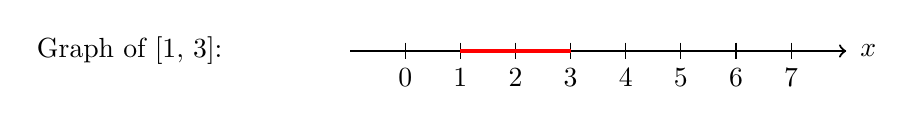
\begin{tikzpicture}[xscale=0.7]
    \draw[->, thick] (-1,0) -- (8,0);
    \foreach \x in  {0,...,7}
    \draw[shift={(\x,0)},color=black] (0pt,3pt) -- (0pt,-3pt);
    \foreach \x in {0,...,7}
    \draw[shift={(\x,0)},color=black] (0pt,0pt) -- (0pt,-3pt) node[below] {$\x$};
    \draw (8.4,0.1pt) node {$x$};
    \draw (-5,0.1pt) node {Graph of $[1,\,3]$:};
    \draw[{[-]}, ultra thick, red] (1,0) -- (3,0);
    \end{tikzpicture}
    \end{center}
    %%%%%
    \begin{center}
    \begin{tikzpicture}[xscale=0.7]
    \draw[->, thick] (-1,0) -- (8,0);
    \foreach \x in  {0,...,7}
    \draw[shift={(\x,0)},color=black] (0pt,3pt) -- (0pt,-3pt);
    \foreach \x in {0,...,7}
    \draw[shift={(\x,0)},color=black] (0pt,0pt) -- (0pt,-3pt) node[below] {$\x$};
    \draw (8.4,0.1pt) node {$x$};
    \draw (-5,0.1pt) node {Graph of $(2,\,6)$:};
    \draw[{(-)}, ultra thick, blue] (2,0) -- (6,0);
    \end{tikzpicture}
    \end{center}
To find $[1,\,3] \cap (2,6)$, take the portion of the number lines that two graphs have in common (overlap).
\begin{equation*}
    [1,\,3] \cap (2,6) = (2,\,3]
\end{equation*}
    \begin{center}
    \begin{tikzpicture}[xscale=0.7]
    \draw[->, thick] (-1,0) -- (8,0);
    \foreach \x in  {0,...,7}
    \draw[shift={(\x,0)},color=black] (0pt,3pt) -- (0pt,-3pt);
    \foreach \x in {0,...,7}
    \draw[shift={(\x,0)},color=black] (0pt,0pt) -- (0pt,-3pt) node[below] {$\x$};
    \draw (8.4,0.1pt) node {$x$};
    \draw[{(-]}, ultra thick, green] (2,0) -- (3,0);
    \end{tikzpicture}
    \end{center}
b. The union of the intervals $[1,\,3]$ and $(2,6)$ consists of the numbers that are in either one interval or the other (or both). To find $[1,\,3] \cup (2,6)$, take the portion of the number lines representing the total collection of numbers in two graphs (sum).
\begin{equation*}
    [1,\,3] \cup (2,6) = [1,\,6)
\end{equation*}
    \begin{center}
    \begin{tikzpicture}[xscale=0.7]
    \draw[->, thick] (-1,0) -- (8,0);
    \foreach \x in  {0,...,7}
    \draw[shift={(\x,0)},color=black] (0pt,3pt) -- (0pt,-3pt);
    \foreach \x in {0,...,7}
    \draw[shift={(\x,0)},color=black] (0pt,0pt) -- (0pt,-3pt) node[below] {$\x$};
    \draw (8.4,0.1pt) node {$x$};
    \draw[{[-)}, ultra thick, green] (1,0) -- (6,0);
    \end{tikzpicture}
    \end{center}
% ======== SECTION
\section{Solving a linear inequality}
Solving inequalities is very similar to solving equations with one exception.  we can add, subtract, multiply, or divide on
both sides of the inequality. But if we multiply or divide by a negative number, the symbol will need to be flipped its direction. We will keep that in mind as we solve
inequalities.
% ===== EXAMPLE 3
\begin{exa}
    Solve and graph the solution set on a number line:
    \begin{equation*}
            -2x-4 > x+5
    \end{equation*}
\end{exa}
\begin{align*}
    -2x-4 > x+5&    &   &\text{Add $2x$ to both sides}\\
    -4 > 3x+5&  &   &\text{Subtract 5 from both sides}\\
    -9 > 3x&    &   &\text{Divide both sides by 3}\\
    &   &           &\text{3 is positive, no need to flip}\\
    -3>x&   &   &\text{Our solution}
\end{align*}
Thus, our answer in set-builder notation is $\{x \mid x<-3\}$. The interval notation for this solution set is $(-\infty,\,-3)$. The graph of the solution set is shown as follows:
    \begin{center}
    \begin{tikzpicture}[xscale=0.7]
    \draw[->, thick] (-8,0) -- (2,0);
    \foreach \x in  {-7,...,1}
    \draw[shift={(\x,0)},color=black] (0pt,3pt) -- (0pt,-3pt);
    \foreach \x in {-7,...,1}
    \draw[shift={(\x,0)},color=black] (0pt,0pt) -- (0pt,-3pt) node[below] {$\x$};
    \draw (1.4,0.1pt) node {$x$};
    \draw[{<-)}, ultra thick, blue] (-8,0) -- (-3,0);
    \end{tikzpicture}
    \end{center}
% ======= EXAMPLE 4
\vspace{0.4cm}
\begin{exa}
    Solve and graph the solution set on a number line:
    \begin{equation*}
        3x+1 \le 7x-15
    \end{equation*}
\end{exa}
\begin{align*}
    3x+1 \le 7x-15& &   &\text{Subtract $7x$ from both sides}\\
    -4x+1 \le -15&  &   &\text{Subtract 1 from both sides}\\
    -4x \le -16&    &   &\text{Divide both sides by $-4$}\\
    &   &   &\text{Divide by a negative number, flip the sign!}\\
    x\,\textcolor{red}{ \ge }\,4&   &   &\text{Our answer}
\end{align*}
Our final solution can expressed in set-builder notation and interval notation as $\{x \mid x\ge 4\}$ and $[4,\, +\infty) $, respectively. The graph of solution set is shown as follows
    \begin{center}
    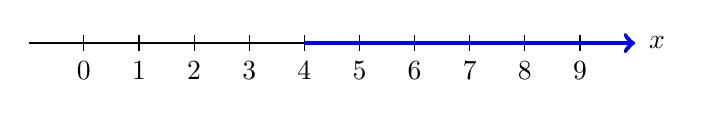
\begin{tikzpicture}[xscale=0.7]
    \draw[->, thick] (-1,0) -- (10,0);
    \foreach \x in  {0,...,9}
    \draw[shift={(\x,0)},color=black] (0pt,3pt) -- (0pt,-3pt);
    \foreach \x in {0,...,9}
    \draw[shift={(\x,0)},color=black] (0pt,0pt) -- (0pt,-3pt) node[below] {$\x$};
    \draw (10.4,0.1pt) node {$x$};
    \draw[{[->}, ultra thick, blue] (4,0) -- (10,0);
    \end{tikzpicture}
    \end{center}
% ======= EXAMPLE 5
\begin{exa}
    Solve and graph the solution set on a number line:
    \begin{equation*}
        \frac{x-4}{2}\ge \frac{x-2}{3}+\frac{5}{6}
    \end{equation*}
\end{exa}
\begin{align*}
    \frac{x-4}{2}\ge \frac{x-2}{3}+\frac{5}{6}& &&\text{LCD of 2,3 and 6 is 6.}\\
    &&&\text{Multiply both sides by 6}\\
    6\biggl(\frac{x-4}{2}\ge \frac{x-2}{3}+\frac{5}{6}\biggr)&
    &   &\text{Distribute and simplify}\\
    3(x-4) \ge 2(x-2) + 1(5)&   &   &\text{Multiply}\\
    3x-12 \ge 2x-4+5&   &   &\text{Combine like terms on LHS}\\
    3x-12 \ge 2x+1& &   &\text{Subtract $2x$ from both sides}\\
    x-12 \ge 1& &   &\text{Add 12 to both sides}\\
    x \ge 13&   &   &\text{Our answer}\\
    \{x \mid x \ge 13\}& &   &\text{Set-builder notation}\\
    [13,\, +\infty)&    &   &\text{Interval notation}
\end{align*}
The graph of solution is shown below
    \begin{center}
    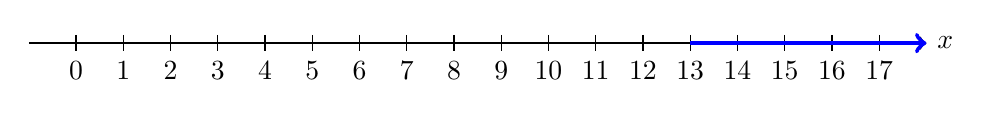
\begin{tikzpicture}[xscale=0.6]
    \draw[->, thick] (-1,0) -- (18,0);
    \foreach \x in  {0,...,17}
    \draw[shift={(\x,0)},color=black] (0pt,3pt) -- (0pt,-3pt);
    \foreach \x in {0,...,17}
    \draw[shift={(\x,0)},color=black] (0pt,0pt) -- (0pt,-3pt) node[below] {$\x$};
    \draw (18.4,0.1pt) node {$x$};
    \draw[{[->}, ultra thick, blue] (13,0) -- (18,0);
    \end{tikzpicture}
    \end{center}
% ======= SECTION
\section{Special inequalities}
Similar to the linear equations, we can reach to a true a statement, like $0<1$, while solving a linear inequality. In this case, the solution set is all real numbers $\{x \mid x\text{ is a real number}\}$ or $(-\infty,\,+\infty)$.\\
Likewise, if we get a false statement, like $0>1$, the solution set is $\{\,\}$ or $\phi$.
% ====== EXAMPLE 
\begin{exa}
    Solve each inequality:
    \begin{enumerate}[\bfseries a.]
        \item $3(x+1) > 3x+2$
        \item $x+1 \le x-1$.
    \end{enumerate}
\end{exa}
a.
\begin{align*}
    3(x+1) > 3x+2&  &   &\text{Simplify LHS}\\
    3x+3 > 3x+2&    &   &\text{Subtract $3x$ from both sides}\\
    3>2&    &   &\text{A true statement}\\
    \{x \mid x \in \mathbb{R}\}& &   &\text{Our solution set in set-builder notation}\\
    (-\infty,\,+\infty)&    &   &\text{Or in interval notation}
\end{align*}
b.
\begin{align*}
    x+1 \le x-1&    &   &\text{Subtract $x$ from both sides}\\
    1 \le -1&   &   &\text{A false statement}\\
    \phi& &   &\text{Our solution}
\end{align*}
% ====== SECTION
\section{Absolute value inequalities}
When an inequality has an absolute value we will have to remove the absolute value in order to graph the solution or give interval notation. The way we remove the absolute value depends on the direction of the inequality symbol.

\vspace{0.2cm}
\textbf{Consider} $\bm{|x|<1}$:\\
Absolute value is defined as distance from zero. Another way to read this inequality would be the distance from zero is less than 1. So on a number line we will shade all points that are less than 1 units away from zero.
    \begin{center}
    \begin{tikzpicture}[xscale=0.7]
    \draw[->, thick] (-6,0) -- (6,0);
    \foreach \x in  {-5,...,5}
    \draw[shift={(\x,0)},color=black] (0pt,3pt) -- (0pt,-3pt);
    \foreach \x in {-5,...,5}
    \draw[shift={(\x,0)},color=black] (0pt,0pt) -- (0pt,-3pt) node[below] {$\x$};
    \draw (6.4,0.1pt) node {$x$};
    \draw[{(-)}, ultra thick, blue] (-1,0) -- (1,0);
    \end{tikzpicture}
    \end{center}
When the absolute value is less than a number will will remove the absolute value by changing the problem to a three part inequality, with the negative value on the left and the positive value on the right. So $|x| < 1$ becomes $− 1 < x < 1$, as the graph above illustrates.

\vspace{0.2cm}
\textbf{Now consider} $\bm{|x| >1}$: \\
Absolute value is defined as distance from zero. Another way to read this inequality would be the distance from zero is greater than 1. So on the number line we shade all points that are more than 1 units away from zero.
    \begin{center}
    \begin{tikzpicture}[xscale=0.7]
    \draw[->, thick] (-6,0) -- (6,0);
    \foreach \x in  {-5,...,5}
    \draw[shift={(\x,0)},color=black] (0pt,3pt) -- (0pt,-3pt);
    \foreach \x in {-5,...,5}
    \draw[shift={(\x,0)},color=black] (0pt,0pt) -- (0pt,-3pt) node[below] {$\x$};
    \draw (6.4,0.1pt) node {$x$};
    \draw[{<-)}, ultra thick, blue] (-6,0) -- (-1,0);
    \draw[{(->}, ultra thick, blue] (1,0) -- (6,0);
    \end{tikzpicture}
    \end{center}
When the absolute value is greater than a number we will remove the absolute value and get two inequalities: the first inequality looking just like the problem with no absolute value, the second flipping the inequality symbol and changing the value to a negative. So $|x| > 1$ becomes $x > 1$ or $x < − 1$, as the graph
above illustrates.
\begin{tcolorbox}[title=How to solve an absolute value inequalities,
colback=blue!5!white,
colframe=blue!75!black,
fonttitle=\bfseries]
First Isolate the absolute value term.
    \begin{itemize}
        \item If $|u|< a$ then $-a< u <a$.
        \item If $|u|>a$ then $u<-a$ or $u>a$.
    \end{itemize}
These rules are valid if $<$ is replaced by $\le$ or $>$ is replaced by $\ge$. 
\end{tcolorbox}
% ===== EXAMPLE 7
\begin{exa}
    Solve and graph the solution set on a number line:
    \begin{equation*}
            |x-2|<5
    \end{equation*}
\end{exa}
The absolute value has already been isolated. Thus,
\begin{align*}
    -5<x-2<5&  &&\text{Add 2 to all sides}\\
    -3<x<7&  &&\text{Our solution}
\end{align*}
Thus, the solution set is $\{ x \mid -3<x<7\}$ or using interval notation we have $(-3,\,7)$. The graph of the solution is illustrated as follows
    \begin{center}
    \begin{tikzpicture}[xscale=0.6]
    \draw[->, thick] (-5,0) -- (9,0);
    \foreach \x in  {-4,...,8}
    \draw[shift={(\x,0)},color=black] (0pt,3pt) -- (0pt,-3pt);
    \foreach \x in {-4,...,8}
    \draw[shift={(\x,0)},color=black] (0pt,0pt) -- (0pt,-3pt) node[below] {$\x$};
    \draw (9.4,0.1pt) node {$x$};
    \draw[{(-)}, ultra thick, blue] (-3,0) -- (7,0);
    \end{tikzpicture}
    \end{center}
% ====== EXAMPLE 8
\begin{exa}
    Solve and graph the solution set on a number line:
    \begin{equation*}
            |4x-5|-5\ge 6
    \end{equation*}
\end{exa}
\begin{align*}
    |4x-5|-5\ge 6&  &   &\text{Isolate the absolute value}\\
    |4x-5| \ge 11&  &   &
\end{align*}
Because of $\ge$ sign we have two inequalities:
\begin{align*}
    4x-5 \le -11&  &&\text{or} &   &4x-5 \ge 11\\
    %
    4x \le -6&  &&\text{or} &   &4x \ge 16\\
    %
    x \le -\frac{6}{4}&  &&\text{or} &   &x \ge \frac{16}{4}\\
    x \le -\frac{3}{2}&  &&\text{or} &   &x \ge 4
\end{align*}
So our solution set is $\left\{x \mid  x\le -\frac{3}{2}\ \text{or}\ x\ge 4 \right\}$ or using interval notation $\left(-\infty,-\frac{3}{2}\, \right] \cup [\,4,+\infty)$. The graph is shown below
    \begin{center}
    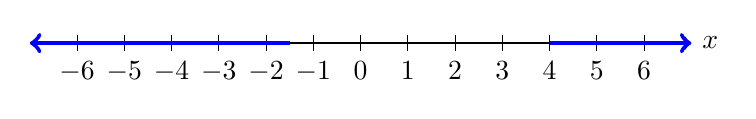
\begin{tikzpicture}[xscale=0.6]
    \draw[->, thick] (-7,0) -- (7,0);
    \foreach \x in  {-6,...,6}
    \draw[shift={(\x,0)},color=black] (0pt,3pt) -- (0pt,-3pt);
    \foreach \x in {-6,...,6}
    \draw[shift={(\x,0)},color=black] (0pt,0pt) -- (0pt,-3pt) node[below] {$\x$};
    \draw (7.4,0.1pt) node {$x$};
    \draw[{[->}, ultra thick, blue] (4,0) -- (7,0);
    \draw[{<-]}, ultra thick, blue] (-7,0) -- (-1.5,0);
    \end{tikzpicture}
    \end{center}